\documentclass[titlepage]{ujarticle}
\usepackage{listings}
\usepackage{jlisting}
\usepackage{ascmac}
\usepackage[dvipdfmx]{graphicx}
\usepackage[top=30truemm,bottom=30truemm,left=25truemm,right=25truemm]{geometry}
\lstset{
	basicstyle={\ttfamily},
	identifierstyle={\small},
	commentstyle={\smallitshape},
	keywordstyle={\small\bfseries},
	ndkeywordstyle={\small},
	stringstyle={\small\ttfamily},
	frame={tb},
	breaklines=true,
	columns=[l]{fullflexible},
	numbers=left,
	xrightmargin=0zw,
	xleftmargin=3zw,
	numberstyle={\scriptsize},
	stepnumber=1,
	numbersep=1zw,
	lineskip=-0.5ex
}

%opening
\title{組み込みソフトウェア工学 課題レポート}
\author{19G463 土居高輔}
\date{2020年2月13日提出}

\begin{document}
\maketitle
\section{問題}
	\ 2人一組で協力して,歩行者用信号機の点灯パターンを実装せよ.青信号は黄色のLEDで代用する.図57を参考に,ピン4に黄色のLEDを,ピン2に赤色のLEDを接続すること(無論,抵抗を入れるのを忘れないこと. \par
	\vspace{\baselineskip}
\section{今回作成したプログラムのソースコードについて}
	\ 今回作成したプログラムのソースコード, TrafficLight.hexは以下の通りである。 \par
	\begin{lstlisting}[caption = TrafficLight.pl, label = program1]
	#ifdef __USE_CMSIS
	#include "LPC8xx.h"
	#endif
	
	#include <cr_section_macros.h>
	#include "type.h"
	
	void SwitchMatrix_Init();
	
	int main(void) {
		SwitchMatrix_Init();
		
		// PIO0_2: output
		LPC_GPIO_PORT->DIR0 |= (1<<2);
		// PIO0_4: output
		LPC_GPIO_PORT->DIR0 |= (1<<4);
		
		// Force the counter to be placed into memory
		volatile static int i = 0 ;
		volatile static int j = 0 ;
		
		// Enter an infinite loop, just incrementing a counter
		while(1) {
			// Toggle PIO0_2
			LPC_GPIO_PORT->NOT0 = 1<<2;	
			for (i=0; i<1000000; i++);
			
			// Yellow_Light_Flash
			for (i=0; i<10; i++) {
				for (j=0; j<100000; j++);
				LPC_GPIO_PORT->NOT0 = 1<<2;
			}
		
			// Red_TurnOn
			LPC_GPIO_PORT->NOT0 = 1<<4;
			for (i=0; i<1000000; i++);
		}
		return 0 ;
	}
	\end{lstlisting}
	\vspace{\baselineskip}
	\ ソースコードの説明をする。 \par
	\begin{lstlisting}[caption = 13~16行目, label = program1]
	// PIO0_2: output
	LPC_GPIO_PORT->DIR0 |= (1<<2);
	// PIO0_4: output
	LPC_GPIO_PORT->DIR0 |= (1<<4);
	\end{lstlisting}
	\vspace{\baselineskip}
	\ 13~16行目、PIO0\_2とPIO0\_4にインタラクト出来るように設定する。 \par
	\vspace{\baselineskip}
	\begin{lstlisting}[caption = 19~20行目, label = program1]
	volatile static int i = 0 ;
	volatile static int j = 0 ;
	\end{lstlisting}
	\vspace{\baselineskip}
	\ 19~20行目、while内で使用するi,jの定義を行う。 \par
	\vspace{\baselineskip}
	\begin{lstlisting}[caption = 23~37行目, label = program1]
	while(1) {
		// Toggle PIO0_2
		LPC_GPIO_PORT->NOT0 = 1<<2;	
		for (i=0; i<1000000; i++);
		
		// Yellow_Light_Flash
		for (i=0; i<10; i++) {
			for (j=0; j<100000; j++);
			LPC_GPIO_PORT->NOT0 = 1<<2;
		}
		
		// Red_TurnOn
		LPC_GPIO_PORT->NOT0 = 1<<4;
		for (i=0; i<1000000; i++);
	}
	\end{lstlisting}
	\vspace{\baselineskip}
	\ 23~37行目、繰り返したい動作内容を記述する。 \par
	\vspace{\baselineskip}
	\begin{lstlisting}[caption = 25~26行目, label = program1]
	// Toggle PIO0_2
	LPC_GPIO_PORT->NOT0 = 1<<2;	
	for (i=0; i<1000000; i++);
	\end{lstlisting}
	\vspace{\baselineskip}
	\ 25~26行目、まず青信号の点灯状態を再現するために、PIO0\_2のトグルを切り替えfor文で待ちを作る。 \par
\newpage
	\vspace{\baselineskip}
	\begin{lstlisting}[caption = 29~32行目, label = program1]
	// Yellow_Light_Flash
	for (i=0; i<10; i++) {
		for (j=0; j<100000; j++);
		LPC_GPIO_PORT->NOT0 = 1<<2;
	}
	\end{lstlisting}
	\vspace{\baselineskip}
	\ 29~32行目、点滅を再現するために少し待ったあとPIO0\_2のトグルを切り替え続ける。 \par
	\vspace{\baselineskip}
	\begin{lstlisting}[caption = 35~36行目, label = program1]
	// Red_TurnOn
	LPC_GPIO_PORT->NOT0 = 1<<4;
	for (i=0; i<1000000; i++);
	\end{lstlisting}
	\vspace{\baselineskip}
	\ 35~36行目、点滅が終わった後、PIO0\_4のトグルを切り替え赤信号の再現をする。 \par
	\vspace{\baselineskip}
\section{配線や動作が分かる写真・動画} 
	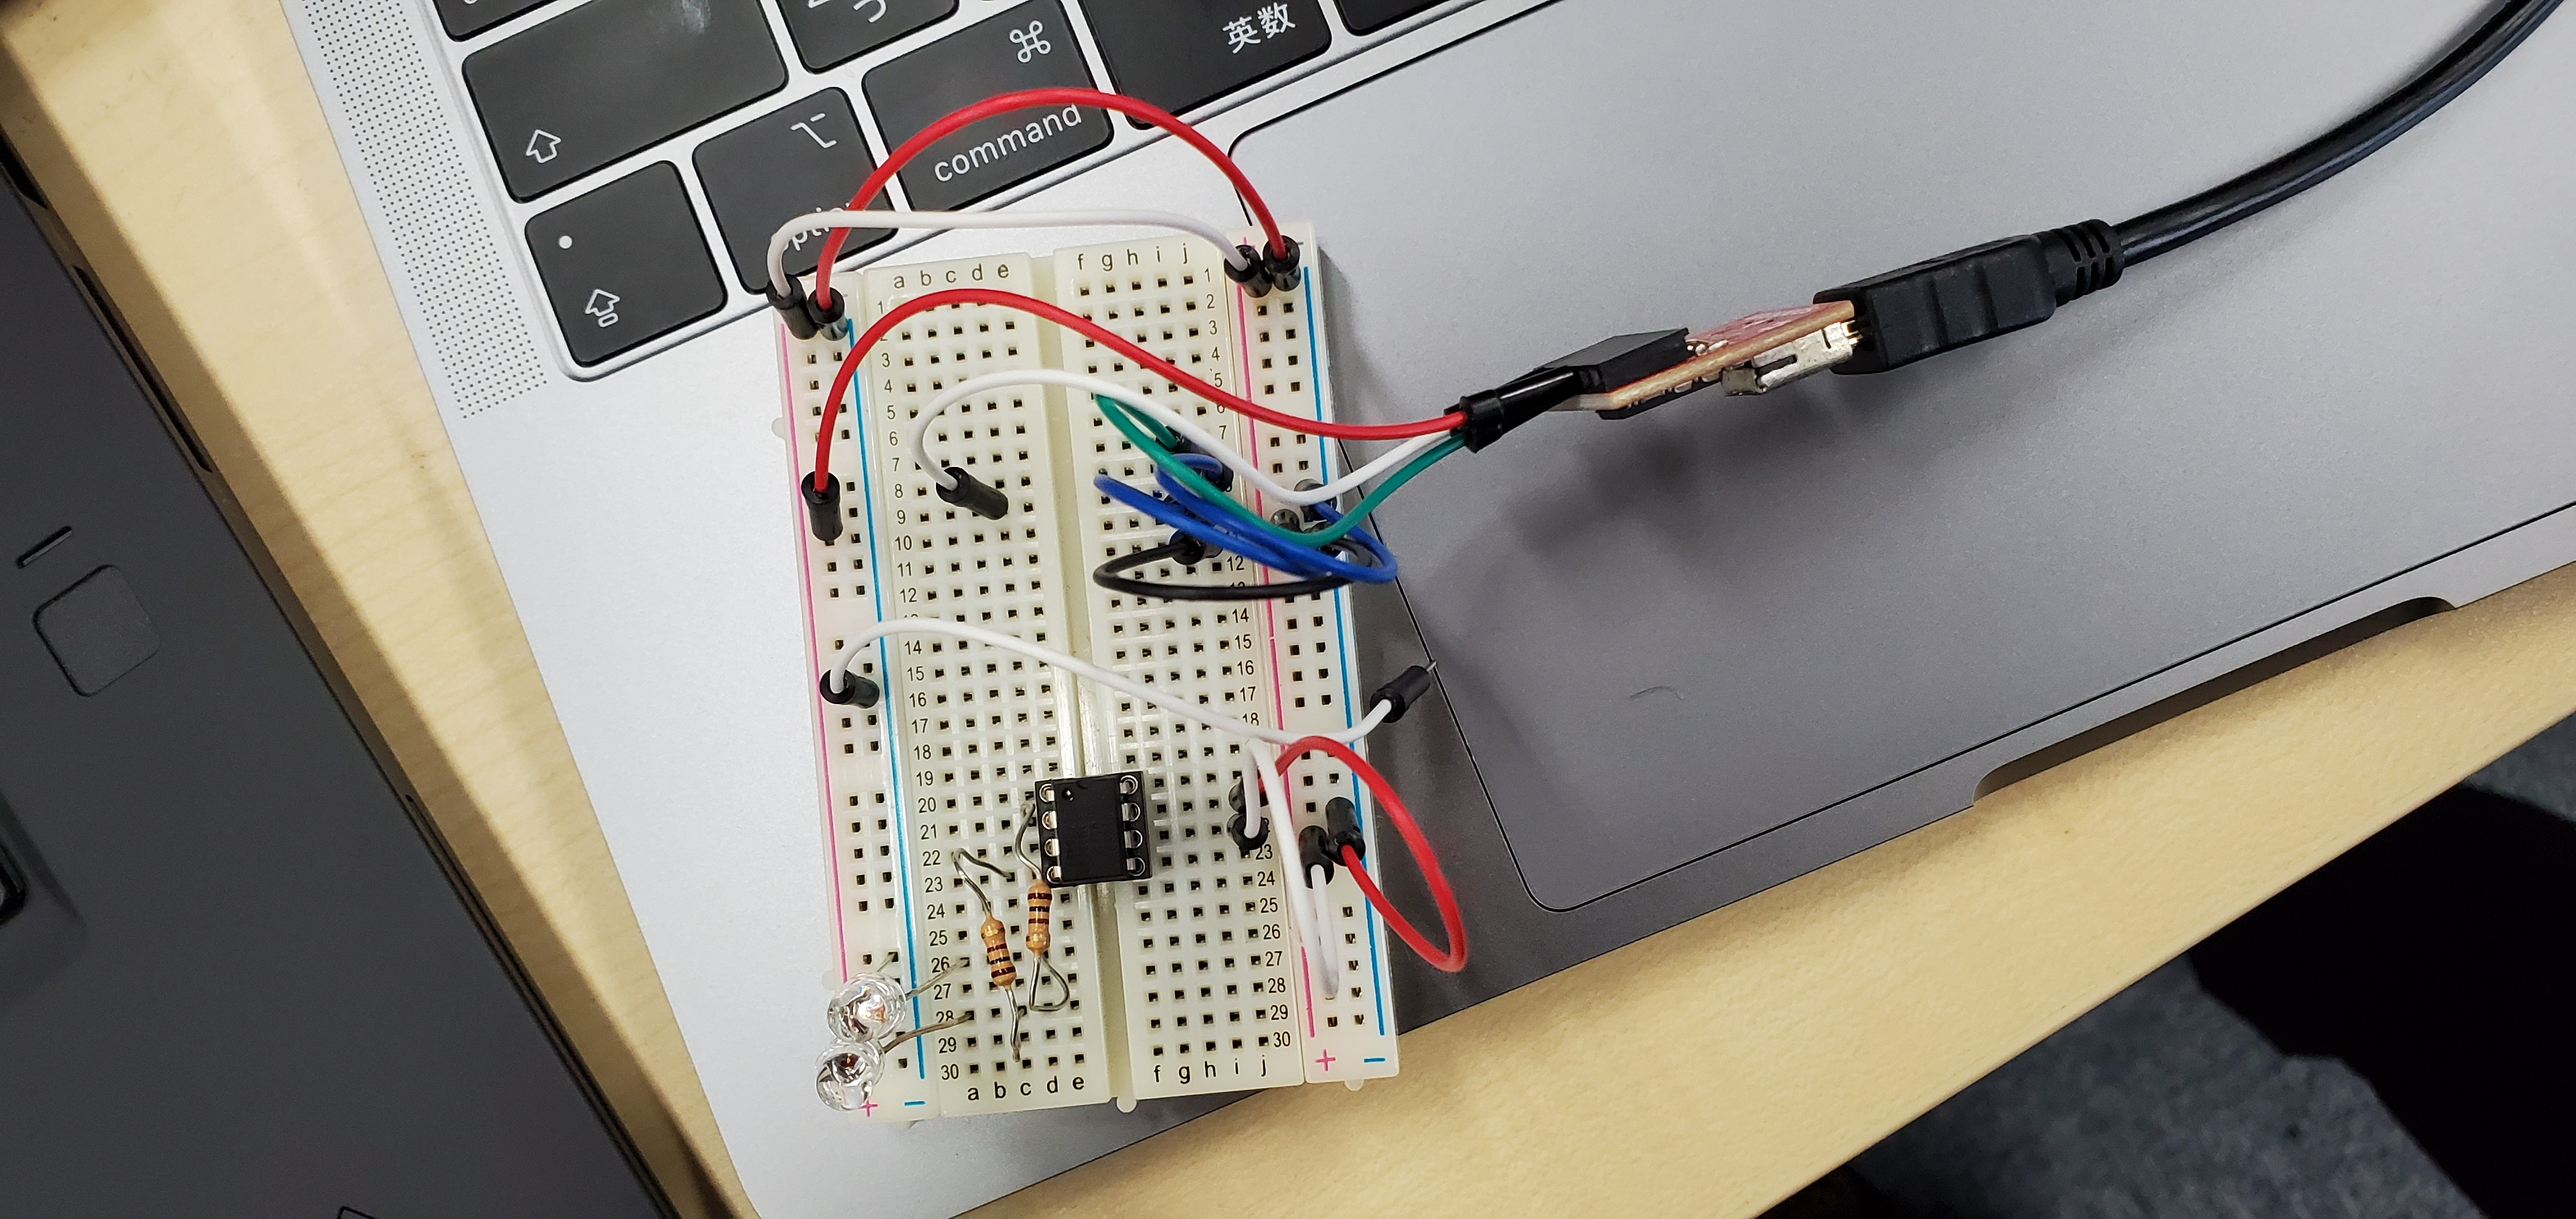
\includegraphics[width=16cm]{1.jpg} \par
	\vspace{\baselineskip}
	\ 動画はフォルダ内のExp\_Movie.mp4を参照してください。 \par
\newpage
\section{感想}
	\ 今回初めてマイコンを用いて組み込みソフトウェアを実装しましたが、PCのUSBポートの相性が悪いため自PCで実験出来なかったことが唯一の心残りです。LEDを点灯・点滅させる簡単なプログラムでしたが、組み込みソフトウェアの実装方法を理解することが出来たので、とても実になった実験でした。今後、組み込み系のプログラムを実装する際には、今回の実験を思い出して頑張ってみようと思います。

\end{document}